%% ============================================================================
%% §4.3.1 ASIC Backend  --  Genus + Innovus
%% Unified narrative; numbers updated to match Peixing's RTL cycle count.
%% ============================================================================
\subsubsection{ASIC Backend: Genus Synthesis and Innovus P\&R}
\label{sec:hw:backend:asic}

The RTL is synthesised with Cadence Genus against the FreePDK45 standard-cell library. Three on-chip memories from the top-level diagram (Figure~\ref{fig:npu_top}) are retargeted for the ASIC: the A/O RAM is realised as an OpenRAM SRAM macro to keep activation accesses dense and low-power; the partial-sum staging register file inside the Post-Process unit is realised as a second OpenRAM SRAM macro; the WGT RAM remains a combinational ROM synthesised from the INT8 weight constants, because FreePDK45 does not ship an SRAM compiler entry sized for the 1\,MB weight memory in this PDK. The Param RAM and Layer Config RAM are small enough to synthesise into standard cells. Synthesis runs at a 5.0\,ns target period. Results are in Table~\ref{tab:syn_results}.

\begin{table}[H]
\centering
\caption{Genus Synthesis Results}
\label{tab:syn_results}
\begin{tabularx}{0.85\textwidth}{l X}
\toprule
\textbf{Metric} & \textbf{Value} \\
\midrule
Target clock period   & 5.0\,ns (200\,MHz) \\
Worst slack (WNS)     & +0.177\,ns \\
Total cells           & 88{,}018 \\
Total area (cells only) & 334{,}956\,$\mu$m$^2$ \\
SRAM macros           & 2 (A/O buffer 97\,K\,$\mu$m$^2$ + partial-sum 66\,K\,$\mu$m$^2$) \\
Critical path         & A/O buffer read $\rightarrow$ SA tile multiplier $\rightarrow$ adder tree $\rightarrow$ Post-Process register \\
\bottomrule
\end{tabularx}
\end{table}

The netlist is then placed and routed in Cadence Innovus on a 720$\times$720\,$\mu$m$^2$ floorplan, shrunk from an initial 800$\times$700 once timing closed. The two SRAM macros are placed manually so the SA dataflow stays compact, and the clock tree uses non-default routing (\texttt{CTS\_2W1S} on leaf nets, \texttt{CTS\_2W2S} on trunks with VSS shielding) to hold skew under 70\,ps. Before LEF import, \texttt{fix\_sram\_lef.py} strips the over-conservative M3/M4 obstructions from the OpenRAM LEF and snaps off-grid pin coordinates to the 0.005\,$\mu$m manufacturing grid; without this step the SRAM dout pins on M3 have no legal via3/M4 escape and the router produces $\sim$480 DRC SHORT/SPACING violations. The final post-route metrics are in Table~\ref{tab:pnr_results} and the layout in Figure~\ref{fig:asic_floorplan}.

\begin{table}[H]
\centering
\caption{Innovus Post-Route Results}
\label{tab:pnr_results}
\begin{tabularx}{\textwidth}{l X}
\toprule
\textbf{Category} & \textbf{Result} \\
\midrule
Core floorplan        & 720$\times$720 $\mu$m$^2$ (518{,}400 $\mu$m$^2$) \\
Placement density     & 59.5\,\% \\
Setup WNS             & +0.089\,ns (MET) \\
Hold WNS              & +0.437\,ns (MET) \\
Setup / Hold TNS      & 0 / 0 \\
DRC violations        & 0 \\
Connectivity          & no problems or warnings \\
Antenna               & no violations \\
Total power           & 96.32\,mW (Switching 43.76, Internal 24.6, Leakage 3.0, Macro 24.9) \\
Cycles per inference  & 19{,}175{,}557 \\
Throughput            & 10.43 FPS @ 200 MHz \\
Energy per inference  & 9.24\,$\mu$J \\
\bottomrule
\end{tabularx}
\end{table}

\begin{figure}[H]
  \centering
  \begin{subfigure}{0.48\textwidth}
    \centering
    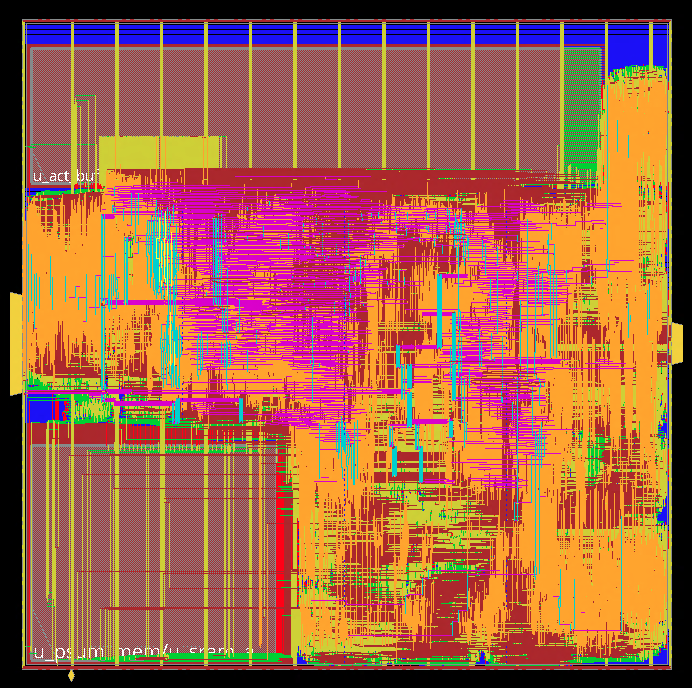
\includegraphics[width=\linewidth]{Fig/mfn_v3_pr.png}
    \caption{Full die view (720$\times$720 $\mu$m$^2$).}
    \label{fig:asic_v3_full}
  \end{subfigure}
\hfill
  \begin{subfigure}{0.48\textwidth}
    \centering
    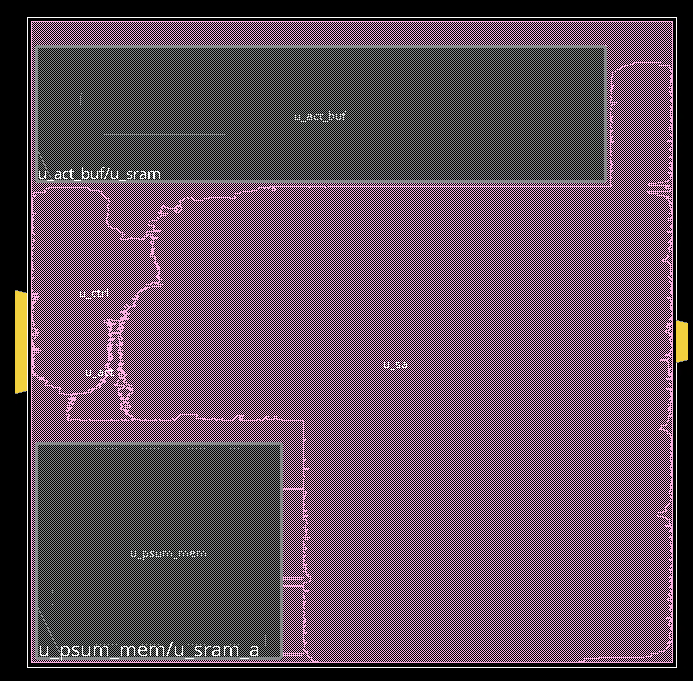
\includegraphics[width=\linewidth]{Fig/mfn_v3_pr_part.png}
    \caption{Detail view: SA + SRAM macros + controller cells.}
    \label{fig:asic_v3_detail}
  \end{subfigure}
  \caption[Innovus post-route layout.]{Final Innovus post-route layout. Two OpenRAM SRAM macros (A/O buffer left, partial-sum buffer right) bracket the central SA placement.}
  \label{fig:asic_floorplan}
\end{figure}

The CTS report (Figure~\ref{fig:asic_cts}) shows balanced clock arrival times across the die with insertion-delay $\mu = 0.348$\,ns, $\sigma = 0.009$\,ns and skew 0.067\,ns.

\begin{figure}[H]
  \centering
  \begin{subfigure}{0.8\textwidth}
    \centering
    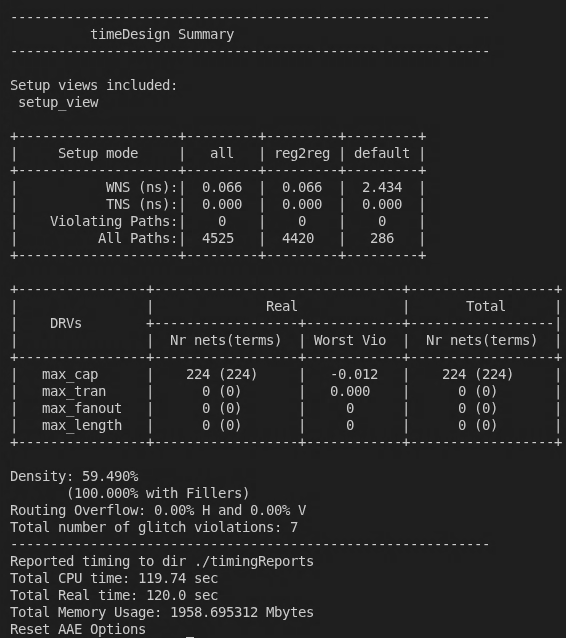
\includegraphics[width=\linewidth]{Fig/mfn_v3_pr_postCTS.png}
    \caption{Post-CTS placement and clock buffers.}
    \label{fig:asic_postcts}
  \end{subfigure} \\[8pt]
  \begin{subfigure}{0.8\textwidth}
    \centering
    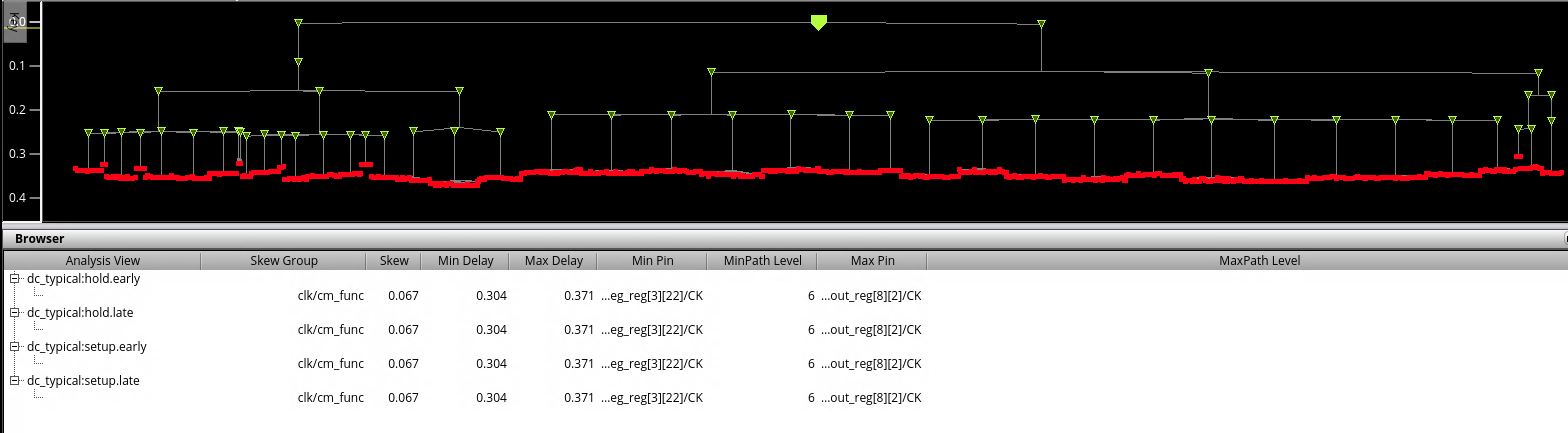
\includegraphics[width=\linewidth]{Fig/mfn_v3_pr_clocks_tree.png}
    \caption{Clock-tree topology and balanced fanout.}
    \label{fig:asic_clk_tree}
  \end{subfigure}
  \caption[Clock-tree synthesis result.]{Clock-tree synthesis result. Skew 0.067\,ns, insertion-delay $\mu = 0.348$\,ns, $\sigma = 0.009$\,ns.}
  \label{fig:asic_cts}
\end{figure}

With WNS $= +0.089$\,ns on the 5.0\,ns target, the critical path measures $T_\text{crit} = 4.911$\,ns. The achievable frequency and the resulting throughput and energy are then

\begin{equation}
F_\text{max} \;=\; \frac{1}{T_\text{crit}} \;=\; \frac{1}{4.911~\text{ns}} \;\approx\; 203.6~\text{MHz},
\label{eq:fmax}
\end{equation}
\begin{equation}
\text{FPS} \;=\; \frac{F_\text{clk}}{C_\text{inf}} \;=\; \frac{200{,}000{,}000}{19{,}175{,}557} \;\approx\; 10.43~\text{frames/s},
\label{eq:fps}
\end{equation}
\begin{equation}
T_\text{inf} \;=\; \frac{C_\text{inf}}{F_\text{clk}} \;\approx\; 95.88~\text{ms}, \quad E_\text{inf} = P_\text{total}\cdot T_\text{inf} \;\approx\; 9.24~\mu\text{J}.
\label{eq:energy}
\end{equation}

The Innovus reports (Figures~\ref{fig:asic_timing_pair} and \ref{fig:asic_route_area}) confirm these numbers and show the 720$\times$720 die routes without congestion hotspots at 59.5\,\% placement density. The power breakdown (Figure~\ref{fig:asic_power}) is dominated by switching activity in the SA, as expected when the $1\times1$ engine fires every cycle at 200\,MHz.

\begin{figure}[H]
  \centering
  \begin{subfigure}{0.48\textwidth}
    \centering
    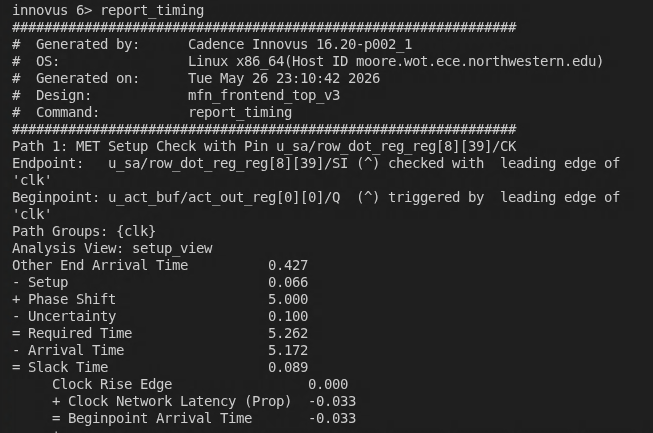
\includegraphics[width=\linewidth]{Fig/mfn_v3_pr_timing.png}
    \caption{Innovus \texttt{report\_timing}: setup WNS +0.089\,ns.}
    \label{fig:asic_timing}
  \end{subfigure}
\hfill
  \begin{subfigure}{0.48\textwidth}
    \centering
    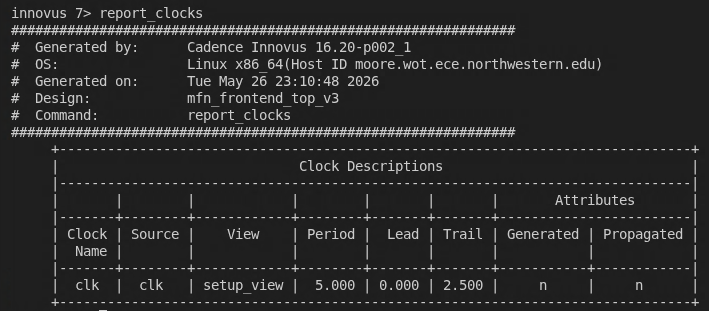
\includegraphics[width=\linewidth]{Fig/mfn_v3_pr_clocks.png}
    \caption{Per-clock summary: 200\,MHz domain.}
    \label{fig:asic_clocks}
  \end{subfigure}
  \caption[Post-route timing and clock-domain reports.]{Post-route timing and clock-domain reports.}
  \label{fig:asic_timing_pair}
\end{figure}

\begin{figure}[H]
  \centering
  \begin{subfigure}{0.48\textwidth}
    \centering
    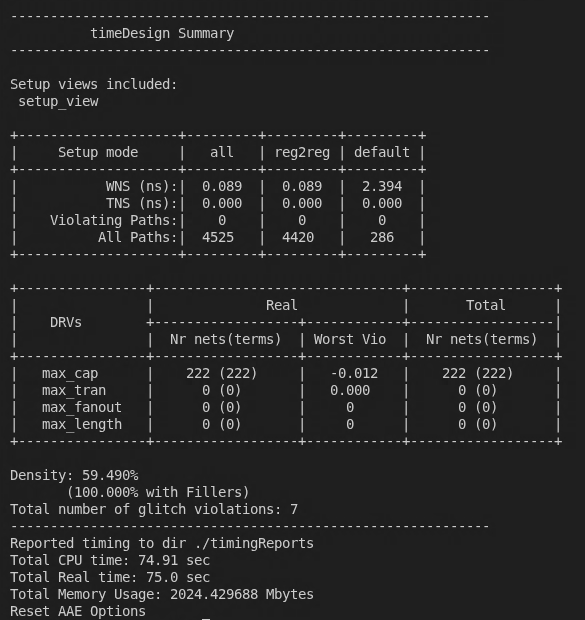
\includegraphics[width=\linewidth]{Fig/mfn_v3_pr_opstRoute.png}
    \caption{Post-route view (\texttt{optsRoute}).}
    \label{fig:asic_optroute}
  \end{subfigure}
\hfill
  \begin{subfigure}{0.48\textwidth}
    \centering
    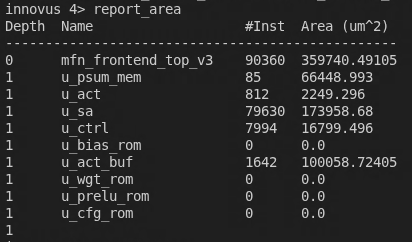
\includegraphics[width=\linewidth]{Fig/mfn_v3_pr_area.png}
    \caption{Area / utilisation report.}
    \label{fig:asic_area}
  \end{subfigure}
  \caption[Routing and area utilisation.]{Routing and area utilisation: zero DRC violations, 59.5\,\% density.}
  \label{fig:asic_route_area}
\end{figure}

\begin{figure}[H]
  \centering
  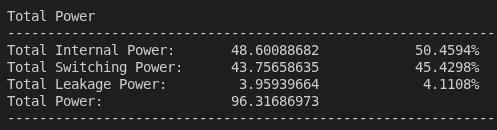
\includegraphics[width=0.7\textwidth]{Fig/mfn_v3_pr_power.png}
  \caption[Innovus post-route power report.]{Innovus post-route power report: total 96.32\,mW, dominated by switching power in the SA at 200\,MHz.}
  \label{fig:asic_power}
\end{figure}
